\documentclass[11pt,a4paper]{article}

\usepackage[a4paper,margin=1in]{geometry}
\usepackage{amsmath}
\usepackage{amssymb}
\usepackage{booktabs}
\usepackage{array}
\usepackage{longtable}
\usepackage{graphicx}
\usepackage{float}
\usepackage{placeins}
\usepackage{graphicx}
\usepackage{float}
\usepackage{placeins}
\usepackage{hyperref}
\usepackage{enumitem}
\usepackage{hyperref}
\usepackage{enumitem}
\usepackage{titlesec}
\usepackage{listings}
\usepackage{xcolor}

\hypersetup{
colorlinks=true,
linkcolor=blue,
urlcolor=blue
}

\lstset{
language=Python,
basicstyle=\ttfamily\small,
keywordstyle=\color{blue},
commentstyle=\color{green!50!black},
stringstyle=\color{red},
numbers=left,
numberstyle=\tiny,
stepnumber=1,
breaklines=true,
frame=single,
showstringspaces=false
}

\renewcommand{\arraystretch}{1.4}

\begin{document}
\raggedbottom

\setlength{\textfloatsep}{10pt}
\setlength{\floatsep}{8pt}
\setlength{\intextsep}{8pt}

\clubpenalty=10000
\widowpenalty=10000
\displaywidowpenalty=10000

\begin{center}

{\Large \textbf{Shiv Nadar University Chennai}}

\vspace{0.3cm}

\begin{tabular}{|p{4cm}|p{8cm}|p{2cm}|}
\hline
Degree \& Branch &
B.Tech Artificial Intelligence \& Data Science &
Semester V\\
\hline
Subject Code \& Name &
CS3807 -- Deep Learning Laboratory &
AY: 2026--27\\
\hline
\end{tabular}

\vspace{0.7cm}

{\Large \textbf{Experiment 2}}

\vspace{0.2cm}

{\large \textbf{Implementation of a Multi-Layer Perceptron (MLP) for Multi-Class Image Classification}}

\end{center}

\section*{1. Objective}

The objective of this experiment is to understand the working principle of a Multi-Layer Perceptron (MLP) and implement one using TensorFlow/Keras for multi-class image classification. The Fashion-MNIST dataset is used to train and evaluate the network. The experiment also aims to study the process of image preprocessing (flattening, normalization and one-hot encoding), analyse the learning behaviour of the network through training and validation curves, evaluate the classifier using standard performance metrics such as Accuracy, Precision, Recall and F1-score, and subsequently perform automated hyperparameter optimization using Randomized Search in order to obtain an improved model configuration.

\section*{2. Background Theory}

A Multi-Layer Perceptron is a class of feedforward Artificial Neural Network consisting of an input layer, one or more hidden layers and an output layer. Unlike the Single Layer Perceptron studied in Experiment 1, which can only solve linearly separable problems, the Multi-Layer Perceptron introduces hidden layers together with non-linear activation functions, enabling the network to approximate complex, non-linear decision boundaries. Each neuron in a given layer is fully connected to every neuron in the preceding layer, and information flows strictly in the forward direction during inference.

Training an MLP involves two major phases. During the forward pass, the input signal is propagated through the network, layer by layer, until the output layer produces a probability distribution over the target classes. During the backward pass, the error between the predicted output and the actual label is computed using a loss function, and this error is propagated backwards through the network using the backpropagation algorithm. The gradients obtained through backpropagation are then used by an optimizer to update the weights and biases of every layer so as to progressively reduce the loss.

\subsection*{Mathematical Formulation}

For a network with $L$ layers, the pre-activation output of layer $l$ is given by

\[
z^{(l)} = W^{(l)} a^{(l-1)} + b^{(l)}
\]

and the corresponding activation is

\[
a^{(l)} = f\left(z^{(l)}\right)
\]

where

\begin{itemize}
\item $a^{(l-1)}$ denotes the activation vector produced by the previous layer, with $a^{(0)}=\mathbf{x}$ representing the flattened, normalized input image of dimension 784.
\item $W^{(l)}$ denotes the weight matrix connecting layer $l-1$ to layer $l$.
\item $b^{(l)}$ denotes the bias vector of layer $l$.
\item $f(\cdot)$ denotes the non-linear activation function of layer $l$.
\item $z^{(l)}$ denotes the pre-activation (weighted sum) of layer $l$.
\end{itemize}

The final, output layer produces class probabilities using the Softmax function

\[
\hat{y}_i = \frac{e^{z_i}}{\displaystyle\sum_{j=1}^{10} e^{z_j}}, \qquad i = 1,2,\dots,10
\]

where $z_i$ is the pre-activation value corresponding to class $i$ at the output layer, and $\hat{y}_i$ is the predicted probability of class $i$.

Since the problem involves multi-class classification with one-hot encoded target labels, the network is trained by minimizing the Categorical Cross-Entropy loss

\[
L = -\sum_{i=1}^{10} y_i \log(\hat{y}_i)
\]

where $y_i$ is the true (one-hot encoded) label for class $i$ and $\hat{y}_i$ is the predicted probability for class $i$.

The weights of every layer are updated using gradient descent, where the gradient of the loss with respect to each weight is obtained through backpropagation

\[
W^{(l)}_{new} = W^{(l)}_{old} - \eta \, \frac{\partial L}{\partial W^{(l)}}
\]

\[
b^{(l)}_{new} = b^{(l)}_{old} - \eta \, \frac{\partial L}{\partial b^{(l)}}
\]

where

\begin{itemize}
\item $\eta$ is the learning rate.
\item $\dfrac{\partial L}{\partial W^{(l)}}$ and $\dfrac{\partial L}{\partial b^{(l)}}$ are the gradients of the loss with respect to the weights and biases of layer $l$, computed using the chain rule.
\end{itemize}

In this experiment, the gradient-based updates are carried out using adaptive optimizers, namely Adam and RMSprop, which maintain per-parameter learning rates based on the first and second moments of the gradients, resulting in faster and more stable convergence compared to plain Stochastic Gradient Descent.

The recommended baseline architecture used in this experiment is

\begin{center}
784 $\rightarrow$ Dense(128, ReLU) $\rightarrow$ Dense(64, ReLU) $\rightarrow$ Dense(10, Softmax)
\end{center}

\subsection*{Activation Functions}

An activation function introduces non-linearity into the network, allowing an MLP to learn complex mapping functions that a purely linear model cannot represent. In this experiment, several activation functions are used across the baseline model, the hyperparameter search space and the final optimized model.

\[
\text{ReLU: } f(z) = \max(0,z)
\]

\[
\text{Tanh: } f(z) = \frac{e^{z}-e^{-z}}{e^{z}+e^{-z}}
\]

\[
\text{Sigmoid: } f(z) = \frac{1}{1+e^{-z}}
\]

\[
\text{Softmax: } f(z_i) = \frac{e^{z_i}}{\displaystyle\sum_{j} e^{z_j}}
\]

The Rectified Linear Unit (ReLU) is computationally efficient and mitigates the vanishing gradient problem, which makes it the default choice for hidden layers of the baseline MLP. The Hyperbolic Tangent (Tanh) function, which was selected by the hyperparameter search for the hidden layers of the optimized model, produces zero-centered outputs in the range $(-1,1)$, often leading to smoother gradient flow than the Sigmoid function. The Softmax function is used exclusively at the output layer to convert the raw output scores into a valid probability distribution over the ten classes.

\vspace{0.15cm}

\begin{center}
\begin{tabular}{|c|c|p{7cm}|}
\hline
\textbf{Activation Function} & \textbf{Output Range} & \textbf{Typical Application}\\
\hline
ReLU & $[0,\infty)$ & Hidden Layers of the Baseline MLP\\
\hline
Tanh & $(-1,1)$ & Hidden Layers of the Optimized MLP\\
\hline
Sigmoid & $(0,1)$ & Candidate Activation in Hyperparameter Search\\
\hline
Softmax & $(0,1)$ & Output Layer -- Multi-class Classification\\
\hline
\end{tabular}
\end{center}

\vspace{0.3cm}

Although ReLU, Tanh and Sigmoid were all included as candidate activation functions in the hyperparameter search space, the automated search identified Tanh as the activation function that produced the best cross-validated performance for the hidden layers, and it was consequently used in the optimized model.

\section*{3. Dataset Description}

The experiment uses the \textbf{Fashion-MNIST Dataset}, a widely used benchmark dataset in the deep learning community, consisting of grayscale images of clothing articles. It is intended as a drop-in, more challenging replacement for the original MNIST handwritten digit dataset.

\vspace{0.3cm}

\begin{center}
\begin{tabular}{|p{5cm}|p{7cm}|}
\hline
\textbf{Property} & \textbf{Value}\\
\hline
Dataset Name & Fashion-MNIST Dataset\\
\hline
Source & Keras Datasets (\texttt{tensorflow.keras.datasets})\\
\hline
Training Images & 60{,}000\\
\hline
Testing Images & 10{,}000\\
\hline
Image Size & $28 \times 28$ (Grayscale)\\
\hline
Flattened Feature Vector & 784\\
\hline
Target Classes & 10\\
\hline
Missing Values & None\\
\hline
Learning Type & Supervised Learning\\
\hline
Problem Type & Multi-class Classification\\
\hline
\end{tabular}
\end{center}

\vspace{0.15cm}

\textbf{Target Classes}

\begin{center}
\begin{tabular}{|c|p{9cm}|}
\hline
\textbf{Class Label} & \textbf{Description}\\
\hline
0 & T-shirt/Top\\
\hline
1 & Trouser\\
\hline
2 & Pullover\\
\hline
3 & Dress\\
\hline
4 & Coat\\
\hline
5 & Sandal\\
\hline
6 & Shirt\\
\hline
7 & Sneaker\\
\hline
8 & Bag\\
\hline
9 & Ankle Boot\\
\hline
\end{tabular}
\end{center}

\vspace{0.3cm}

The dataset contains no missing values and each of the ten classes is represented by exactly 6{,}000 training images, resulting in a perfectly balanced class distribution. This balance ensures that the trained network is not biased towards any particular category during learning. Each image, originally provided as a $28\times28$ pixel matrix, must be transformed into a flat 784-dimensional feature vector prior to being supplied to the fully connected (Dense) layers of the MLP.

\section*{4. Image Preprocessing}

Since Dense layers of an MLP require a one-dimensional feature vector rather than a two-dimensional image matrix, every $28\times28$ image is flattened into a vector of length 784

\[
28 \times 28 = 784
\]

For instance, a small $2\times2$ image matrix is flattened in row-major order as follows

\[
\begin{bmatrix}
10 & 20\\
30 & 40
\end{bmatrix}
\rightarrow
[10,\,20,\,30,\,40]
\]

The following preprocessing steps were carried out prior to model construction.

\begin{enumerate}
\item Loaded the Fashion-MNIST dataset using \texttt{tensorflow.keras.datasets}.
\item Displayed ten sample images together with their class labels.
\item Flattened every $28\times28$ image into a 784-dimensional feature vector.
\item Normalized pixel intensities from the range $[0,255]$ to $[0,1]$ by dividing by 255.
\item Converted the integer class labels into one-hot encoded vectors of length 10 using \texttt{to\_categorical}.
\end{enumerate}

\section*{5. Experimental Procedure}

The experiment was carried out using Python with TensorFlow/Keras in Google Colab. The implementation followed a systematic workflow beginning from dataset loading and ending with automated hyperparameter optimization and final model comparison.

\subsection*{Task 1: Dataset Exploration}

The Fashion-MNIST dataset was loaded directly using \texttt{tensorflow.keras.datasets.fashion\_mnist}. The shapes of the training and testing partitions were verified, the number of classes and class labels were printed, ten representative sample images were displayed along with their true class names, and the class distribution across the training set was plotted.

\textbf{Output}

\begin{itemize}
\item Training Images Shape : (60000, 28, 28)
\item Training Labels Shape : (60000,)
\item Testing Images Shape : (10000, 28, 28)
\item Testing Labels Shape : (10000,)
\item Image Size : 28 x 28
\item Number of Classes : 10
\item Class Labels : [0 1 2 3 4 5 6 7 8 9]
\end{itemize}

\vspace{0.3cm}

The dataset exploration confirmed that the images were correctly loaded and that no missing or corrupted samples were present.

\subsection*{Task 2: Data Preprocessing}

The images were flattened, normalized and one-hot encoded as described in Section 5.

\textbf{Output}

\begin{itemize}
\item Flattened Training Shape : (60000, 784)
\item Flattened Testing Shape : (10000, 784)
\item Encoded Training Shape : (60000, 10)
\item Encoded Testing Shape : (10000, 10)
\end{itemize}

\vspace{0.3cm}

The comparison of tensor shapes before and after preprocessing confirmed that every image was correctly transformed from a $28\times28$ matrix into a flat, normalized 784-dimensional vector, and that every integer label was correctly converted into a 10-dimensional one-hot vector.

\subsection*{Task 3: Model Construction}

A baseline Multi-Layer Perceptron was constructed using the Keras Sequential API with the following architecture.

\begin{itemize}
\item Input Layer : 784 neurons (flattened pixel vector)
\item Hidden Layer 1 : Dense, 128 neurons, ReLU activation
\item Hidden Layer 2 : Dense, 64 neurons, ReLU activation
\item Output Layer : Dense, 10 neurons, Softmax activation
\end{itemize}

The model was compiled using the Adam optimizer, the Categorical Cross-Entropy loss function and Accuracy as the evaluation metric. The \texttt{model.summary()} output confirmed a total of 109{,}386 trainable parameters distributed across the three Dense layers, as reported in Section 8.

\subsection*{Task 4: Model Training}

The baseline model was compiled using

\begin{itemize}
\item Optimizer : Adam
\item Loss : Categorical Cross-Entropy
\item Metric : Accuracy
\end{itemize}

and trained for 20 epochs with a batch size of 32, using 20\% of the training data reserved as a validation split. Training and validation accuracy and loss were recorded after every epoch in order to monitor learning progress and detect signs of overfitting.

\subsection*{Task 5: Model Evaluation}

After training, the baseline model was evaluated on the untouched testing set of 10{,}000 images. The following metrics were computed.

\begin{itemize}
\item Accuracy
\item Precision (weighted average)
\item Recall (weighted average)
\item F1-Score (weighted average)
\item Confusion Matrix
\item Classification Report (per-class precision, recall and F1-score)
\end{itemize}

\subsection*{Task 6: Hyperparameter Optimization and Model Comparison}

Rather than manually selecting the network hyperparameters, an automated Randomized Search was performed using the SciKeras wrapper together with Scikit-learn's \texttt{RandomizedSearchCV}, employing 5-fold cross-validation over a wide search space covering the number of hidden layers, the number of neurons per layer, the learning rate, the batch size, the number of epochs, the optimizer, the activation function and the dropout rate. The best configuration identified by the search was then used to construct and train an optimized MLP, which was evaluated on the testing set and compared against the baseline model.

\section*{6. Source Code}

The complete implementation was carried out in Python using Google Colab and TensorFlow/Keras, following the task-wise structure described in Section 5 (dataset loading, preprocessing, baseline model construction and training, baseline evaluation, automated hyperparameter optimization using RandomizedSearchCV, optimized model construction and training, and final evaluation).

Owing to its length, the complete, executable source code has not been reproduced in full within this report. The complete Google Colab notebook, containing every code cell together with its executed output, is publicly available at the following repository link.

\begin{center}
\url{https://github.com/K-Mithran/Deep-Learning/blob/main/Lab2/DL_2.ipynb}
\end{center}

The major stages of implementation included

\begin{enumerate}
\item Loading the Fashion-MNIST dataset.
\item Performing exploratory data analysis (sample images and class distribution).
\item Flattening, normalizing and one-hot encoding the images.
\item Constructing and training the baseline MLP.
\item Evaluating the baseline model on the testing set.
\item Performing automated hyperparameter optimization using Randomized Search.
\item Constructing and training the optimized MLP using the best hyperparameters.
\item Evaluating the optimized model and comparing it against the baseline.
\end{enumerate}


\section*{7. Hyperparameter Optimization}

Instead of manually selecting the network hyperparameters, an automated search was performed using \textbf{RandomizedSearchCV} together with the SciKeras wrapper, which allows a Keras model to be used as a Scikit-learn compatible estimator. Randomized Search was preferred over an exhaustive Grid Search because the combined search space is extremely large, and Randomized Search allows a representative sample of configurations to be evaluated within a practical time budget while still providing a reliable estimate of the best-performing region of the hyperparameter space.

The following search space was defined for the optimization process.

\begin{center}
\begin{tabular}{|p{5cm}|p{7cm}|}
\hline
\textbf{Hyperparameter} & \textbf{Candidate Values}\\
\hline
Hidden Layers & 1, 2, 3\\
\hline
Hidden Neurons & 32, 64, 128, 256\\
\hline
Learning Rate & 0.1, 0.01, 0.001\\
\hline
Batch Size & 16, 32, 64, 128\\
\hline
Epochs & 10, 20, 30\\
\hline
Optimizer & SGD, Adam, RMSprop\\
\hline
Activation Function & ReLU, Tanh, Sigmoid\\
\hline
Dropout Rate & 0.0, 0.2, 0.5\\
\hline
\end{tabular}
\end{center}

\vspace{0.3cm}

The Randomized Search was configured to sample 15 candidate hyperparameter combinations ($n\_iter=15$), each evaluated using 5-fold cross-validation, resulting in a total of 75 individual model fits. Accuracy was used as the scoring metric, and the random state was fixed at 42 to ensure reproducibility of the sampled configurations.

\begin{center}
\begin{tabular}{|p{6cm}|p{6cm}|}
\hline
\textbf{Search Configuration} & \textbf{Value}\\
\hline
Search Strategy & RandomizedSearchCV\\
\hline
Number of Sampled Configurations & 15\\
\hline
Cross-validation Folds & 5\\
\hline
Total Model Fits & 75\\
\hline
Scoring Metric & Accuracy\\
\hline
Random State & 42\\
\hline
\end{tabular}
\end{center}

\vspace{0.3cm}

Upon completion of the search, the following hyperparameter combination was identified as the best-performing configuration based on the mean cross-validation accuracy.

\begin{center}
\begin{tabular}{|p{6cm}|p{6cm}|}
\hline
\textbf{Hyperparameter} & \textbf{Best Value}\\
\hline
Hidden Layers & 3\\
\hline
Hidden Neurons & 128\\
\hline
Learning Rate & 0.001\\
\hline
Batch Size & 32\\
\hline
Optimizer & RMSprop\\
\hline
Activation Function & Tanh\\
\hline
Epochs & 30\\
\hline
Dropout Rate & 0.2\\
\hline
Best Cross-validation Accuracy & 88.74\%\\
\hline
Optimization Time & 5480.85 seconds ($\approx$91.35 minutes)\\
\hline
\end{tabular}
\end{center}

\vspace{0.3cm}

These best-identified hyperparameters were subsequently used to construct the optimized MLP, consisting of three hidden Dense layers of 128 neurons each with Tanh activation, a Dropout layer with a rate of 0.2 following every hidden layer, and an output Dense layer of 10 neurons with Softmax activation, compiled using the RMSprop optimizer with a learning rate of 0.001.

\section*{8. Experimental Results}

\subsection*{8.1 Dataset Exploration}

The Fashion-MNIST dataset was successfully loaded using the Keras Datasets API. The dataset contains 60{,}000 training images and 10{,}000 testing images, each of size $28\times28$ pixels, spread uniformly across 10 classes.

\begin{center}
\begin{tabular}{|p{6cm}|p{5cm}|}
\hline
\textbf{Property} & \textbf{Observed Value}\\
\hline
Training Images & 60{,}000\\
\hline
Testing Images & 10{,}000\\
\hline
Image Dimensions & $28\times28$\\
\hline
Number of Classes & 10\\
\hline
Missing Values & 0\\
\hline
Flattened Feature Length & 784\\
\hline
\end{tabular}
\end{center}

\vspace{0.15cm}

The dataset was found to be complete, correctly labeled and free of missing values. Every class was represented by exactly 6{,}000 training samples, confirming a perfectly balanced dataset that requires no additional class-balancing technique before training.

\subsection*{8.2 Data Preprocessing Results}

After flattening, every image was transformed from a $28\times28$ matrix into a 784-dimensional feature vector. Pixel intensities, originally in the range $[0,255]$, were normalized to the range $[0,1]$, and the integer class labels were converted into one-hot encoded vectors of length 10.

\begin{center}
\begin{tabular}{|p{6cm}|p{5cm}|}
\hline
\textbf{Stage} & \textbf{Shape}\\
\hline
Flattened Training Features & (60000, 784)\\
\hline
Flattened Testing Features & (10000, 784)\\
\hline
One-hot Encoded Training Labels & (60000, 10)\\
\hline
One-hot Encoded Testing Labels & (10000, 10)\\
\hline
\end{tabular}
\end{center}

\vspace{0.15cm}

This preprocessing step ensured that every image was represented in a format compatible with the Dense (fully connected) layers of the MLP, and that the pixel scale did not disproportionately influence the gradient updates during training.

\subsection*{8.3 Baseline Model}

The baseline MLP was constructed with the architecture 784 $\rightarrow$ Dense(128, ReLU) $\rightarrow$ Dense(64, ReLU) $\rightarrow$ Dense(10, Softmax), compiled using the Adam optimizer with Categorical Cross-Entropy loss.

\begin{center}
\begin{tabular}{|p{6cm}|p{6cm}|}
\hline
\textbf{Layer} & \textbf{Output Shape / Parameters}\\
\hline
Hidden\_Layer\_1 (Dense, ReLU) & (None, 128) -- 100{,}480 params\\
\hline
Hidden\_Layer\_2 (Dense, ReLU) & (None, 64) -- 8{,}256 params\\
\hline
Output\_Layer (Dense, Softmax) & (None, 10) -- 650 params\\
\hline
Total Trainable Parameters & 109{,}386\\
\hline
\end{tabular}
\end{center}

\vspace{0.15cm}

The baseline model was trained for 20 epochs using a batch size of 32, with 20\% of the training data reserved for validation. The training accuracy increased steadily from 82.12\% in the first epoch to 93.36\% by the twentieth epoch, while the training loss decreased from 0.5103 to 0.1746 over the same period. The validation accuracy improved from 85.03\% to a peak in the high 89\% range, stabilizing around 88--89\% for the later epochs, while the validation loss exhibited a mild upward trend after around epoch 9, indicating the onset of slight overfitting as the network continued to fit the training data more closely than the validation data.

\begin{center}
\begin{tabular}{|p{6cm}|p{6cm}|}
\hline
\textbf{Parameter} & \textbf{Value}\\
\hline
Final Training Accuracy (Epoch 20) & 93.36\%\\
\hline
Final Training Loss (Epoch 20) & 0.1746\\
\hline
Final Validation Accuracy (Epoch 20) & 88.99\%\\
\hline
Final Validation Loss (Epoch 20) & 0.3608\\
\hline
Training Time & 97.32 seconds\\
\hline
\end{tabular}
\end{center}

\vspace{0.15cm}

The baseline model was then evaluated on the held-out testing set of 10{,}000 previously unseen images.

\begin{center}
\begin{tabular}{|p{6cm}|c|}
\hline
\textbf{Metric} & \textbf{Value}\\
\hline
Accuracy & 88.09\%\\
\hline
Precision (weighted) & 88.20\%\\
\hline
Recall (weighted) & 88.09\%\\
\hline
F1-Score (weighted) & 88.02\%\\
\hline
\end{tabular}
\end{center}

\vspace{0.15cm}

The per-class classification report revealed that Trouser (99\% precision, 97\% recall), Sandal (99\% precision, 93\% recall) and Bag (97\% precision, 97\% recall) were classified with very high accuracy, since these categories possess visually distinctive shapes. In contrast, the Shirt class obtained the lowest performance (76\% precision, 64\% recall), and was frequently confused with visually similar upper-body garments such as T-shirt/Top, Pullover and Coat, which is an expected and well-documented characteristic of the Fashion-MNIST dataset.

\subsection*{8.4 Optimized Model}

Using the best hyperparameters identified by the Randomized Search (Section 8), the optimized MLP was constructed with three hidden Dense layers of 128 neurons each using Tanh activation, each followed by a Dropout layer with a rate of 0.2, and compiled using the RMSprop optimizer with a learning rate of 0.001.

\begin{center}
\begin{tabular}{|p{6cm}|p{6cm}|}
\hline
\textbf{Layer} & \textbf{Output Shape / Parameters}\\
\hline
Hidden\_Layer\_1 (Dense, Tanh) & (None, 128) -- 100{,}480 params\\
\hline
Dropout (rate = 0.2) & (None, 128) -- 0 params\\
\hline
Hidden\_Layer\_2 (Dense, Tanh) & (None, 128) -- 16{,}512 params\\
\hline
Dropout (rate = 0.2) & (None, 128) -- 0 params\\
\hline
Hidden\_Layer\_3 (Dense, Tanh) & (None, 128) -- 16{,}512 params\\
\hline
Dropout (rate = 0.2) & (None, 128) -- 0 params\\
\hline
Output\_Layer (Dense, Softmax) & (None, 10) -- 1{,}290 params\\
\hline
Total Trainable Parameters & 134{,}794\\
\hline
\end{tabular}
\end{center}

\vspace{0.15cm}

The optimized model was trained for 30 epochs with a batch size of 32 and a 20\% validation split. The training accuracy increased steadily from 78.76\% in the first epoch to 90.33\% by the thirtieth epoch, while the training loss decreased from 0.5844 to 0.2750. The validation accuracy rose from 82.98\% to a final value of 88.85\%, and the validation loss decreased from 0.4638 to a final value of 0.3326. Compared to the baseline model, the training and validation curves of the optimized model remained noticeably closer to each other throughout training, indicating that the additional Dropout regularization was effective in reducing the gap between training and validation performance, thereby limiting overfitting.

\begin{center}
\begin{tabular}{|p{6cm}|p{6cm}|}
\hline
\textbf{Parameter} & \textbf{Value}\\
\hline
Final Training Accuracy (Epoch 30) & 90.33\%\\
\hline
Final Training Loss (Epoch 30) & 0.2750\\
\hline
Final Validation Accuracy (Epoch 30) & 88.85\%\\
\hline
Final Validation Loss (Epoch 30) & 0.3326\\
\hline
Training Time & 157.47 seconds\\
\hline
\end{tabular}
\end{center}

\vspace{0.15cm}

The optimized model was evaluated on the same testing set of 10{,}000 images used for the baseline model.

\begin{center}
\begin{tabular}{|p{6cm}|c|}
\hline
\textbf{Metric} & \textbf{Value}\\
\hline
Accuracy & 88.05\%\\
\hline
Precision (weighted) & 88.18\%\\
\hline
Recall (weighted) & 88.05\%\\
\hline
F1-Score (weighted) & 88.10\%\\
\hline
\end{tabular}
\end{center}

\vspace{0.15cm}

The per-class classification report of the optimized model showed a similar overall pattern to the baseline model, with Trouser (99\% precision, 96\% recall) and Bag (97\% precision, 97\% recall) remaining the best-classified categories. Notably, the Shirt class, which was the weakest class for the baseline model, improved slightly in recall (from 64\% to 71\%) with the optimized model, although its precision decreased marginally (from 76\% to 69\%), suggesting a shift in the decision boundary rather than a uniform improvement across all metrics for that class.

\subsection*{8.5 Baseline vs Optimized: Performance Comparison}

\begin{center}
\begin{tabular}{|p{4cm}|c|c|}
\hline
\textbf{Metric} & \textbf{Baseline} & \textbf{Optimized}\\
\hline
Accuracy & 88.09\% & 88.05\%\\
\hline
Precision & 88.20\% & 88.18\%\\
\hline
Recall & 88.09\% & 88.05\%\\
\hline
F1-Score & 88.02\% & 88.10\%\\
\hline
Training Time & 97.32 s & 157.47 s\\
\hline
\end{tabular}
\end{center}

\vspace{0.15cm}

The comparison shows that the optimized model achieved a testing accuracy and precision that were marginally lower than the baseline model, while its F1-Score was marginally higher. In practical terms, the two models performed almost identically on the held-out testing set, with differences well under half a percentage point across all four metrics. This result is discussed further in Section 11.

\section*{9. Performance Summary}

\begin{center}
\begin{tabular}{|p{7cm}|p{5cm}|}
\hline
Training Images & 60{,}000\\
\hline
Testing Images & 10{,}000\\
\hline
Flattened Feature Length & 784\\
\hline
Number of Classes & 10\\
\hline
Baseline Architecture & 784-128-64-10\\
\hline
Baseline Optimizer & Adam\\
\hline
Baseline Epochs & 20\\
\hline
Baseline Testing Accuracy & 88.09\%\\
\hline
Hyperparameter Search Method & RandomizedSearchCV (5-fold CV)\\
\hline
Best CV Accuracy & 88.74\%\\
\hline
Optimized Architecture & 784-128-128-128-10 (Dropout 0.2)\\
\hline
Optimized Optimizer & RMSprop (lr = 0.001)\\
\hline
Optimized Epochs & 30\\
\hline
Optimized Testing Accuracy & 88.05\%\\
\hline
\end{tabular}
\end{center}

\section*{10. Generated Plots with Interpretation}

%%%%%%%%%%%%%%%%%%%%%%%%%%%%%%%%%%%%%%%%%%%%%%%%%%%%%%%%%%%%%%

\subsection*{10.1 Sample Images}

\begin{figure}[H]
\centering
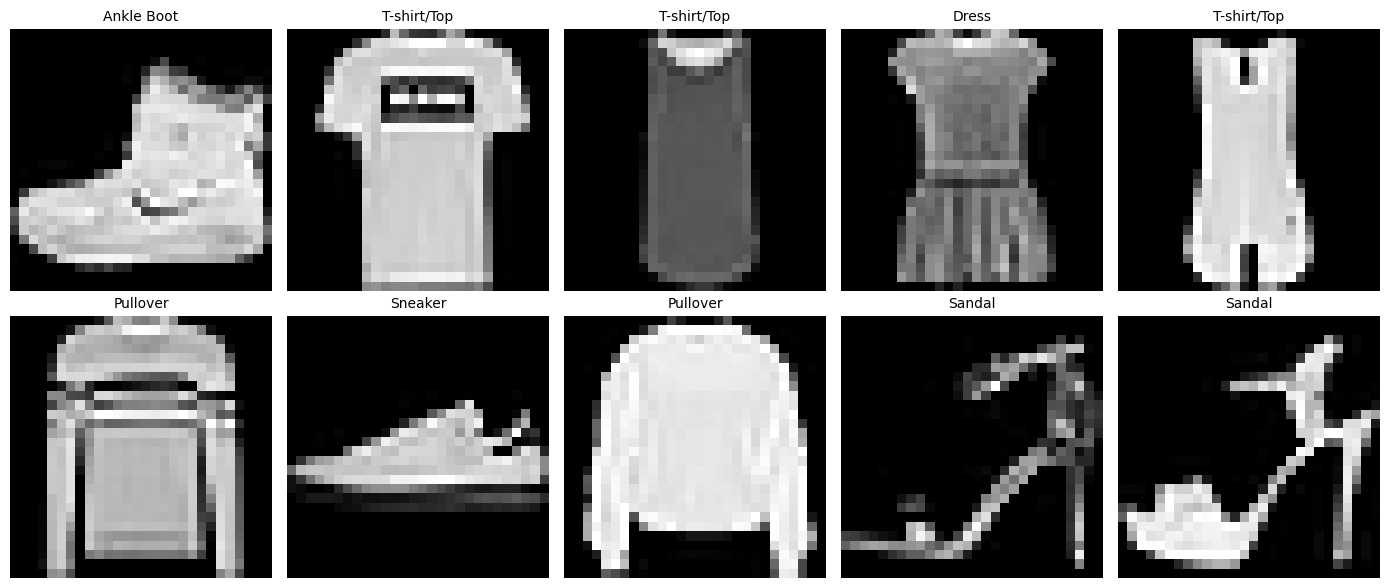
\includegraphics[width=0.95\textwidth]{plot1.png}
\caption{Ten Sample Images from the Fashion-MNIST Dataset with True Class Labels}
\end{figure}

The sample images illustrate the visual diversity of the ten clothing categories present in the Fashion-MNIST dataset. Several categories, such as Trouser and Sandal, possess distinctive silhouettes, whereas categories such as Shirt, Pullover and Coat share considerable visual overlap, which explains the relatively lower classification performance observed for these classes.

\vspace{0.15cm}

%%%%%%%%%%%%%%%%%%%%%%%%%%%%%%%%%%%%%%%%%%%%%%%%%%%%%%%%%%%%%%

\subsection*{10.2 Class Distribution}

\begin{figure}[H]
\centering
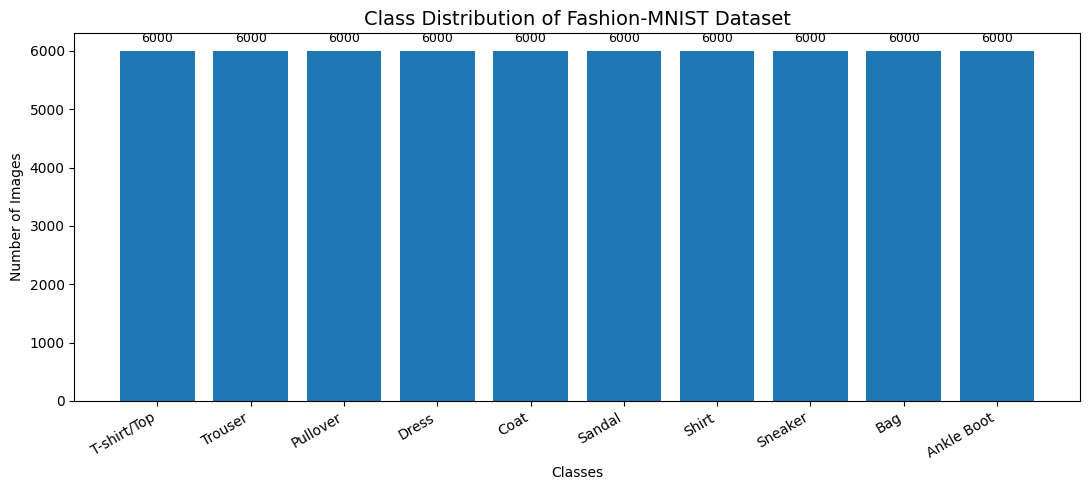
\includegraphics[width=0.85\textwidth]{plot2.png}
\caption{Class Distribution of the Fashion-MNIST Training Dataset}
\end{figure}

The bar chart confirms that each of the ten classes contains exactly 6{,}000 training images, indicating a perfectly balanced dataset. This balance ensures that the network is not biased towards predicting any particular class more frequently due to unequal representation in the training data.

\vspace{0.15cm}

%%%%%%%%%%%%%%%%%%%%%%%%%%%%%%%%%%%%%%%%%%%%%%%%%%%%%%%%%%%%%%

\subsection*{10.3 Baseline Confusion Matrix}

\begin{figure}[H]
\centering
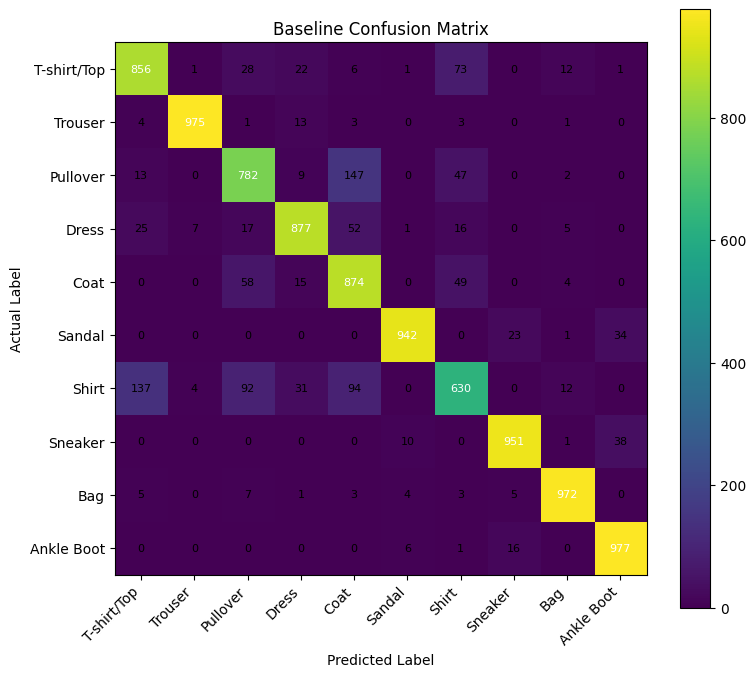
\includegraphics[width=0.68\textwidth]{plot3.png}
\caption{Confusion Matrix of the Baseline MLP on the Testing Set}
\end{figure}

The confusion matrix of the baseline model shows that the majority of predictions lie along the diagonal, confirming a high overall classification accuracy. The most prominent off-diagonal confusion occurs between the Shirt class and the T-shirt/Top, Pullover and Coat classes, which is consistent with the visual similarity among these upper-body garment categories.

\vspace{0.15cm}

%%%%%%%%%%%%%%%%%%%%%%%%%%%%%%%%%%%%%%%%%%%%%%%%%%%%%%%%%%%%%%

\subsection*{10.4 Baseline Training Accuracy vs Epoch}

\begin{figure}[H]
\centering
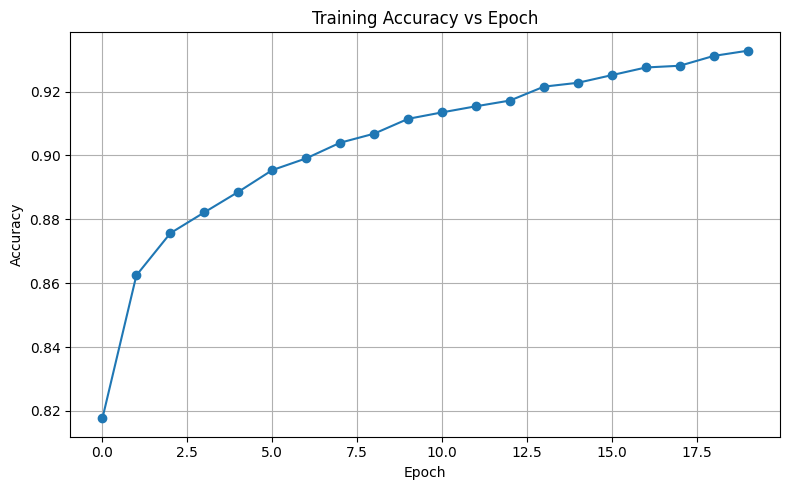
\includegraphics[width=0.66\textwidth]{plot4.png}
\caption{Training Accuracy vs Epoch -- Baseline Model}
\end{figure}

The training accuracy of the baseline model increases consistently across all 20 epochs, rising from approximately 82\% to over 93\%. The smooth, monotonically increasing curve indicates that the network is steadily learning the mapping between the input pixel vectors and the correct class labels, without any signs of instability during training.

\vspace{0.15cm}

%%%%%%%%%%%%%%%%%%%%%%%%%%%%%%%%%%%%%%%%%%%%%%%%%%%%%%%%%%%%%%

\subsection*{10.5 Baseline Validation Accuracy vs Epoch}

\begin{figure}[H]
\centering
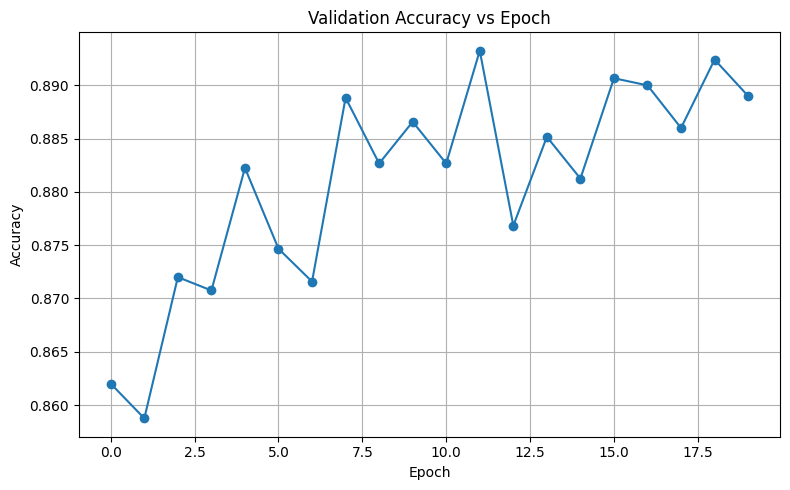
\includegraphics[width=0.66\textwidth]{plot5.png}
\caption{Validation Accuracy vs Epoch -- Baseline Model}
\end{figure}

The validation accuracy rises sharply during the first few epochs and then plateaus around 88--89\%, with minor epoch-to-epoch fluctuations. Unlike the training accuracy, the validation accuracy does not continue to increase towards the later epochs, suggesting that the baseline model begins to overfit the training data after roughly epoch 9 or 10.

\vspace{0.15cm}

%%%%%%%%%%%%%%%%%%%%%%%%%%%%%%%%%%%%%%%%%%%%%%%%%%%%%%%%%%%%%%

\subsection*{10.6 Baseline Training Loss vs Epoch}

\begin{figure}[H]
\centering
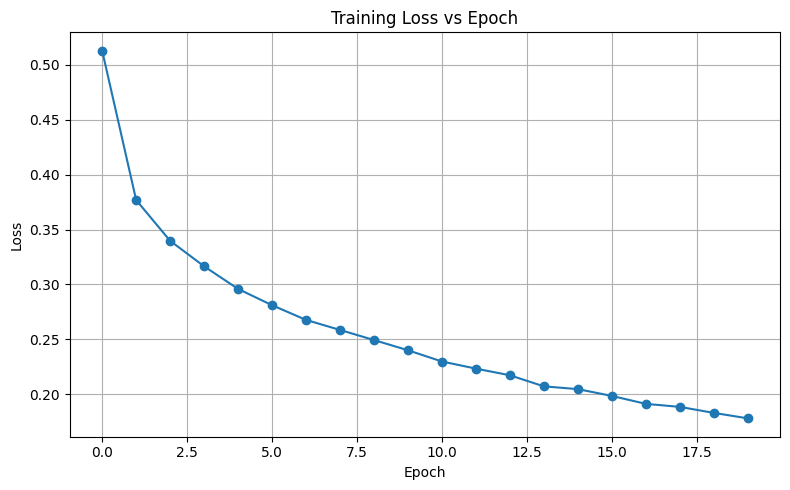
\includegraphics[width=0.66\textwidth]{plot6.png}
\caption{Training Loss vs Epoch -- Baseline Model}
\end{figure}

The training loss decreases smoothly and consistently throughout all 20 epochs, falling from approximately 0.51 to below 0.18. This steady decline demonstrates that the Adam optimizer is effectively minimizing the Categorical Cross-Entropy loss on the training set at every step.

\vspace{0.15cm}

%%%%%%%%%%%%%%%%%%%%%%%%%%%%%%%%%%%%%%%%%%%%%%%%%%%%%%%%%%%%%%

\subsection*{10.7 Baseline Validation Loss vs Epoch}

\begin{figure}[H]
\centering
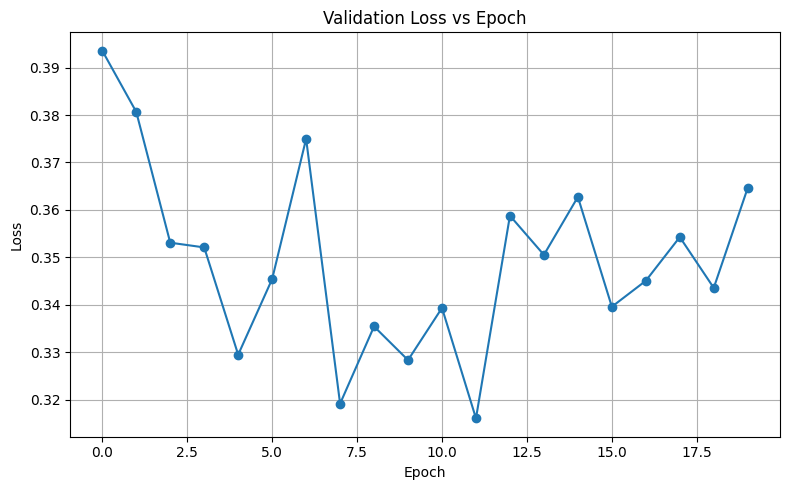
\includegraphics[width=0.66\textwidth]{plot7.png}
\caption{Validation Loss vs Epoch -- Baseline Model}
\end{figure}

Unlike the training loss, the validation loss decreases only for the first few epochs before beginning to fluctuate and gradually trend upward for the remaining epochs. This divergence between the training loss (which keeps decreasing) and the validation loss (which stagnates and rises) is a classic indicator of overfitting in the baseline model, motivating the use of regularization techniques such as Dropout in the optimized model.

\vspace{0.15cm}

%%%%%%%%%%%%%%%%%%%%%%%%%%%%%%%%%%%%%%%%%%%%%%%%%%%%%%%%%%%%%%

\subsection*{10.8 Optimized Model Accuracy}

\begin{figure}[H]
\centering
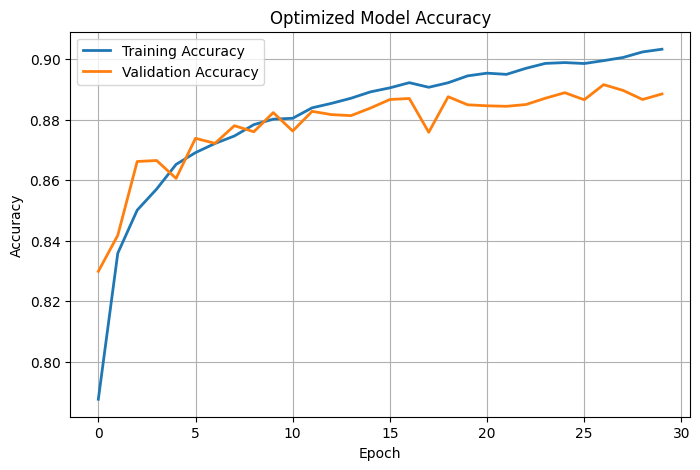
\includegraphics[width=0.66\textwidth]{plot8.png}
\caption{Training and Validation Accuracy vs Epoch -- Optimized Model}
\end{figure}

The training and validation accuracy curves of the optimized model remain much closer together throughout the 30 training epochs compared to the corresponding baseline curves. Both curves rise steadily and converge towards a similar final value near 89--90\%, indicating that the Dropout layers introduced in the optimized architecture successfully reduced the gap between training and validation performance.

\vspace{0.15cm}

%%%%%%%%%%%%%%%%%%%%%%%%%%%%%%%%%%%%%%%%%%%%%%%%%%%%%%%%%%%%%%

\subsection*{10.9 Optimized Model Loss}

\begin{figure}[H]
\centering
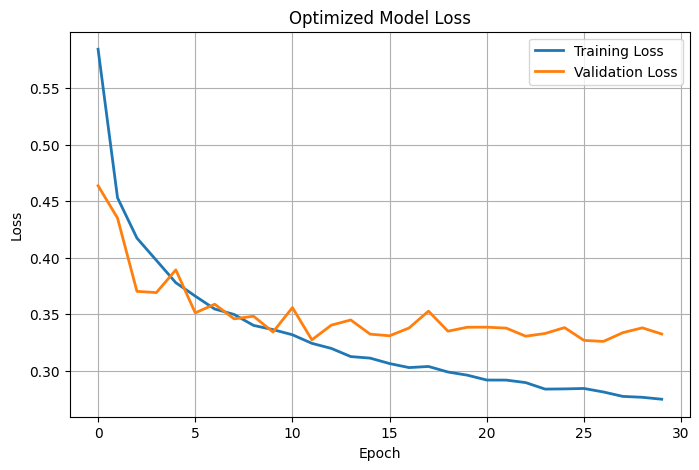
\includegraphics[width=0.66\textwidth]{plot9.png}
\caption{Training and Validation Loss vs Epoch -- Optimized Model}
\end{figure}

The training and validation loss curves of the optimized model decrease together for a longer portion of the training process compared to the baseline model, and the gap between the two curves remains comparatively narrow even towards the final epochs. This behaviour confirms that the combination of additional hidden layers, Dropout regularization and the RMSprop optimizer produced a more stable and better-regularized training process.

\vspace{0.15cm}

%%%%%%%%%%%%%%%%%%%%%%%%%%%%%%%%%%%%%%%%%%%%%%%%%%%%%%%%%%%%%%



\subsection*{10.10 Optimized Model Confusion Matrix}

\begin{figure}[H]
\centering
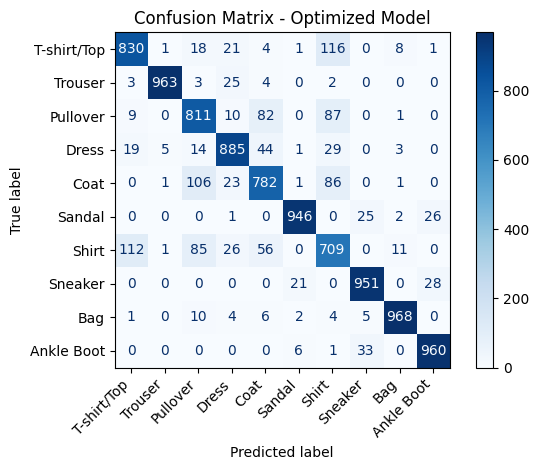
\includegraphics[width=0.72\textwidth]{plot10.png}
\caption{Confusion Matrix of the Optimized MLP on the Testing Set}
\end{figure}

The confusion matrix of the optimized model shows a diagonal pattern very similar to that of the baseline model, with the vast majority of testing samples correctly classified. The Shirt class continues to be the most frequently confused category, being misclassified primarily as T-shirt/Top, Pullover and Coat, indicating that this difficulty stems from the inherent visual ambiguity of the dataset rather than from a deficiency specific to either model architecture.

\section*{11. Discussion}

The Multi-Layer Perceptron demonstrated that a fully connected feedforward network trained on flattened, normalized pixel vectors can classify Fashion-MNIST images effectively, with both the baseline and optimized models reaching a testing accuracy of approximately 88\%. Randomized Search was preferred over an exhaustive Grid Search because the defined search space, spanning eight hyperparameters, would have been computationally prohibitive to evaluate exhaustively; sampling 15 configurations under 5-fold cross-validation instead located a strong region of the space at a fraction of the cost. The search selected 3 hidden layers of 128 neurons, Tanh activation, a Dropout rate of 0.2 and the RMSprop optimizer (learning rate 0.001) as the best configuration, with the number of hidden layers, the activation function and the dropout rate appearing to influence cross-validation accuracy the most.

Notably, the optimized model's testing accuracy (88.05\%) was marginally lower than the baseline's (88.09\%), despite the optimized configuration achieving a higher cross-validation accuracy (88.74\%). This is not a failure of the search: cross-validation accuracy is estimated on resampled training folds and need not transfer exactly to a single fixed test split, the added Dropout trades a little raw fitting capacity for stability, and a difference under half a percentage point lies well within normal run-to-run variation of stochastic training. The real benefit of the optimized model is visible in its accuracy and loss curves, where the training and validation curves track much closer together than in the baseline, indicating reduced overfitting and more reliable generalization behaviour.

Both models found the Shirt class hardest to classify, confusing it mainly with T-shirt/Top, Pullover and Coat. This reflects genuine visual overlap between these garments at $28\times28$ resolution rather than an architectural weakness, and would likely require a spatially-aware model such as a CNN to resolve.

\section*{12. Conclusion}

A Multi-Layer Perceptron was implemented in TensorFlow/Keras for multi-class classification on the Fashion-MNIST dataset. After flattening, normalizing and one-hot encoding the images, a baseline MLP (two hidden Dense layers) trained for 20 epochs achieved a testing accuracy of 88.09\%, precision of 88.20\%, recall of 88.09\% and F1-Score of 88.02\%.

RandomizedSearchCV with 5-fold cross-validation was then used to tune the hidden layers, neurons, learning rate, batch size, epochs, optimizer, activation function and dropout rate, identifying a deeper, Dropout-regularized, Tanh-based RMSprop configuration with a cross-validation accuracy of 88.74\%. Retrained with these settings, the optimized model achieved a testing accuracy of 88.05\%, precision of 88.18\%, recall of 88.05\% and F1-Score of 88.10\% -- essentially on par with the baseline, but with a visibly narrower training-validation gap, reflecting improved regularization.

The experiment shows that automated hyperparameter optimization does not always yield a strictly higher test accuracy than a well-designed baseline, but remains valuable for improving training stability and generalization. It also reinforced practical understanding of MLP design, activation functions, image preprocessing, backpropagation-based training and systematic model comparison using standard classification metrics.

\section*{13. References}

\begin{enumerate}

\item Ian Goodfellow,
Yoshua Bengio,
Aaron Courville,
\textit{Deep Learning},
MIT Press,
2016.

\item Christopher M. Bishop,
\textit{Pattern Recognition and Machine Learning},
Springer,
2006.

\item Simon Haykin,
\textit{Neural Networks and Learning Machines},
Pearson Education,
2009.

\item Han Xiao, Kashif Rasul, Roland Vollgraf,
\textit{Fashion-MNIST: a Novel Image Dataset for Benchmarking Machine Learning Algorithms},
2017.

\url{https://github.com/zalandoresearch/fashion-mnist}

\item TensorFlow/Keras Documentation.

\url{https://www.tensorflow.org/guide/keras}

\item Scikit-learn Documentation.

\url{https://scikit-learn.org}

\item SciKeras Documentation.

\url{https://www.adriangb.com/scikeras/}

\end{enumerate}

\vfill

\end{document}